\documentclass{llncs}

\usepackage{listings}
\usepackage{graphicx}
\usepackage{url}

\bibliographystyle{alpha}

% Default settings for listings. %
\lstset{ %
basicstyle=\footnotesize,       % the size of the fonts that are used for the code
numberstyle=\footnotesize,      % the size of the fonts that are used for the line-numbers
numbers=left,                   % where to put the line-numbers
stepnumber=1,                   % the step between two line-numbers. If it's 1 each line will be numbered
numbersep=5pt,                  % how far the line-numbers are from the code
showspaces=false,               % show spaces adding particular underscores
showstringspaces=false,         % underline spaces within strings
showtabs=false,                 % show tabs within strings adding particular underscores
tabsize=2,	                % sets default tabsize to 2 spaces
captionpos=b,                   % sets the caption-position to bottom
breaklines=true,                % sets automatic line breaking
breakatwhitespace=false,        % sets if automatic breaks should only happen at whitespace
escapeinside={\%*}{*)}          % if you want to add a comment within your code
}


\begin{document}

\title{Event-Driven Verification in Dynamic Component Models}

% lets invite Carlos and Birgit - Claas what do you think ??
\author{Jens Dietrich\inst{1} \and Claas Wilke\inst{2}}

\institute{Massey University, Institute of Information Sciences and Technology,\\ Palmerston North, New Zealand \and
Institut f\"ur Software- und Multimediatechnik,\\ Technische Universit\"at Dresden, Germany}

\maketitle


% TODO Info: This work was funded by ... %

\begin{abstract}

We propose ActiveTreaty, a novel contract and verification model suitable for dynamic component systems. ActiveTreaty combines aspects of static and dynamic verification by checking component contracts whenever certain lifecycle events occur. We introduce a role model that supports the flexible, context-dependent management of different aspects of contract management and enforcement. 
A proof-of-concept implementation for the OSGi/Eclipse component model is presented. 

\end{abstract}



\section{Introduction}

In recent years, dynamic component models supporting the dynamic (re-)\-con\-fi\-gu\-ra\-tion of applications have become very successful. Examples include \textit{OSGi} \cite{OSGI} and its derivatives and \textit{.NET} \cite{MSdotNet}. Some of the largest and most complex systems are now based on these models, including \textit{IBM WebSphere} \cite{IBMWebsphere} and \textit{Oracle WebLogic} \cite{OracleWebLogic}. The question arises how these systems can be effectively verified. In practise, static verification techniques are still dominant. This includes the use of compilers and unit testing. Verification is typically performed for single components at built-time. Component containers and runtime environments have little support to verify the integrity of composed systems. For instance, OSGi containers merely check the type safety of classes providing services described by interfaces, and the version compatibility of the components composed. This is based on the implicit assumption that compatibility information between components can be completely described by the combination of service interfaces and dependencies between versioned packages and components. 

In our previous work \cite{Treaty.JOT2009}, we have argued that a more expressive contract language is needed to precisely describe the relationship between collaborating components. This has resulted in \textit{Treaty}, an expressive, component-model independent contract language. Treaty supports alternative contract arrangements (disjunction), collaborations based on resources other than program language types, and therefore contracts that describe different aspects of component compatibility \cite{BeugnardEtAl99} including interface, behavioural and quality of service contracts. It turns out that these features are appropriate to simplify and improve the contract management in applications based on dynamic component systems such as \textit{Eclipse} \cite{Eclipse}. 

The original version of Treaty was static in the sense that contracts are represented by integrity rules. Once a contract is instantiated when collaborating components pair up, contracts are ready to be used for verification. However, Treaty makes no assumptions how they are actually used. On the other hand, dynamic component models like OSGi have well defined lifecycle models that describe the various lifecycle states of components, and the transitions between these states. It is therefore possible to use the events signalling state transitions to trigger contract verification. 

In this paper, we propose an extension to make Treaty this dynamic by including both the events that trigger contract verification, and the actions that are to be performed upon verification  to the contracts. This implies that contracts are represented using event-condition-action rules (ECA rules for short). 

The rest of this paper is organised as follows. In the next section, we review related work. We then sketch the Treaty framework in section \ref{section:treaty}. For a detailed description, the reader is referred to \cite{Treaty.JOT2009}. In section \ref{section:activeTreaty}, we introduce active treaty. Afterwards, the present a prototypical implementation of ActiveTreaty for Eclipse as a case study in section \ref{section:caseStudy}. Section \ref{section:conclusion} concludes this work.

TODO: Probably complete.



\section{Related Work}

% TODO Jens: the next two paragraphs are copied from the TKDE submission, need to ve rephrased

The idea of having contracts between collaborating software artefacts has been pioneered by Meyers work on \textit{design by contract} \cite{DesignByContract,meyerOOSC}. Contracts are added directly to the programming language source code, the artefacts bound by contracts are methods. There is no explicit event handling, contract checks are performed when the methods are invoked. Several authors have adopted these ideas to other programming languages and runtime environments, including the Java Modelling Language (JML) \cite{DBLP:conf/fmco/ChalinKLP05}. Arnout and Meyer  \cite{ArnoutMeyer2003b} have used ``A Posteriori Contracting'' to add contracts to existing software artifacts. This is similar to the introduction of legislator components discussed below.   

Formal contract languages have been used successfully in order to define several kinds of contracts in business computing, including \textit{SLA contracts} \cite{PaschkeDietrich2005}, \textit{business contracts} \cite{Linington04} \cite{Governatori05} \cite{Governatori06} and the provisions for exception handling in \textit{electronic contracts} \cite{SweetDeal}. These languages support complex event handling, in particular through the use of \textit{Event-Condition-Action (ECA) rules}.  

TODO Probably more related work



\section{The Treaty Contract Language}
\label{section:treaty}

In this section, we provide a brief introduction into Treaty. For more details, the reader is referred to \cite{Treaty.JOT2009}. Treaty is a framework to manage different types of contracts in dynamic component systems. It is based on the idea that components interact through connectors by providing and consuming resources. Examples for (dynamic) components are Eclipse plug-ins and OSGi bundles, examples for connectors are Eclipse extensions and extension points, respectively. Contracts describe this interaction. The requirements in these contracts are themselves expressed through resources that are usually provided by the consumer. Examples for this are Java interfaces and XML Schemas. Suppliers of services provide other resources that have to have certain typed relationships with consumer side resources. For instance, they provide classes that must \textit{implement} (consumer-side) 
interfaces and XML documents that must \textit{instantiate} XML Schemas. Treaty contracts consist of these typed relationships or boolean expressions built from these relationships. Besides relationships, simple properties (comparisons) and resource existence conditions can also be expressed. It turns out that this representation is appropriate to express many types of contracts in existing component models. In particular in the case of Eclipse,  both logically complex conditions and contracts using resource types other than Java types are needed. The type system used by Treaty is based on the \textit{resource description framework (RDF)} \cite{RDF} and the \textit{web ontology language (OWL)} \cite{OWL}. I.e., resource, property and relationship types are represented by URIs and reasoning features such as subtype and subproperty reasoning are supported. 

Treaty is suitable for dynamic component models using late binding. This is facilitated by the fact that contracts can be defined without explicit reference to a supplier or a consumer. The missing resources can be referenced by function symbols representing queries to component meta data. Once the supplier or consumer is known (at runtime), the contract is instantiated by executing these queries against the meta data of this component and replacing the functions by the actual resource references. This process is called \textit{binding}. In the Treaty proof-of-concept implementation for Eclipse, these functions are \textit{XPath} expressions that are resolved against the \texttt{plugin.xml} meta data file of the supplier plugin when binding occurs. 
%TODO probably a reference for XPath?%

\begin{figure}[t]
  \centering
  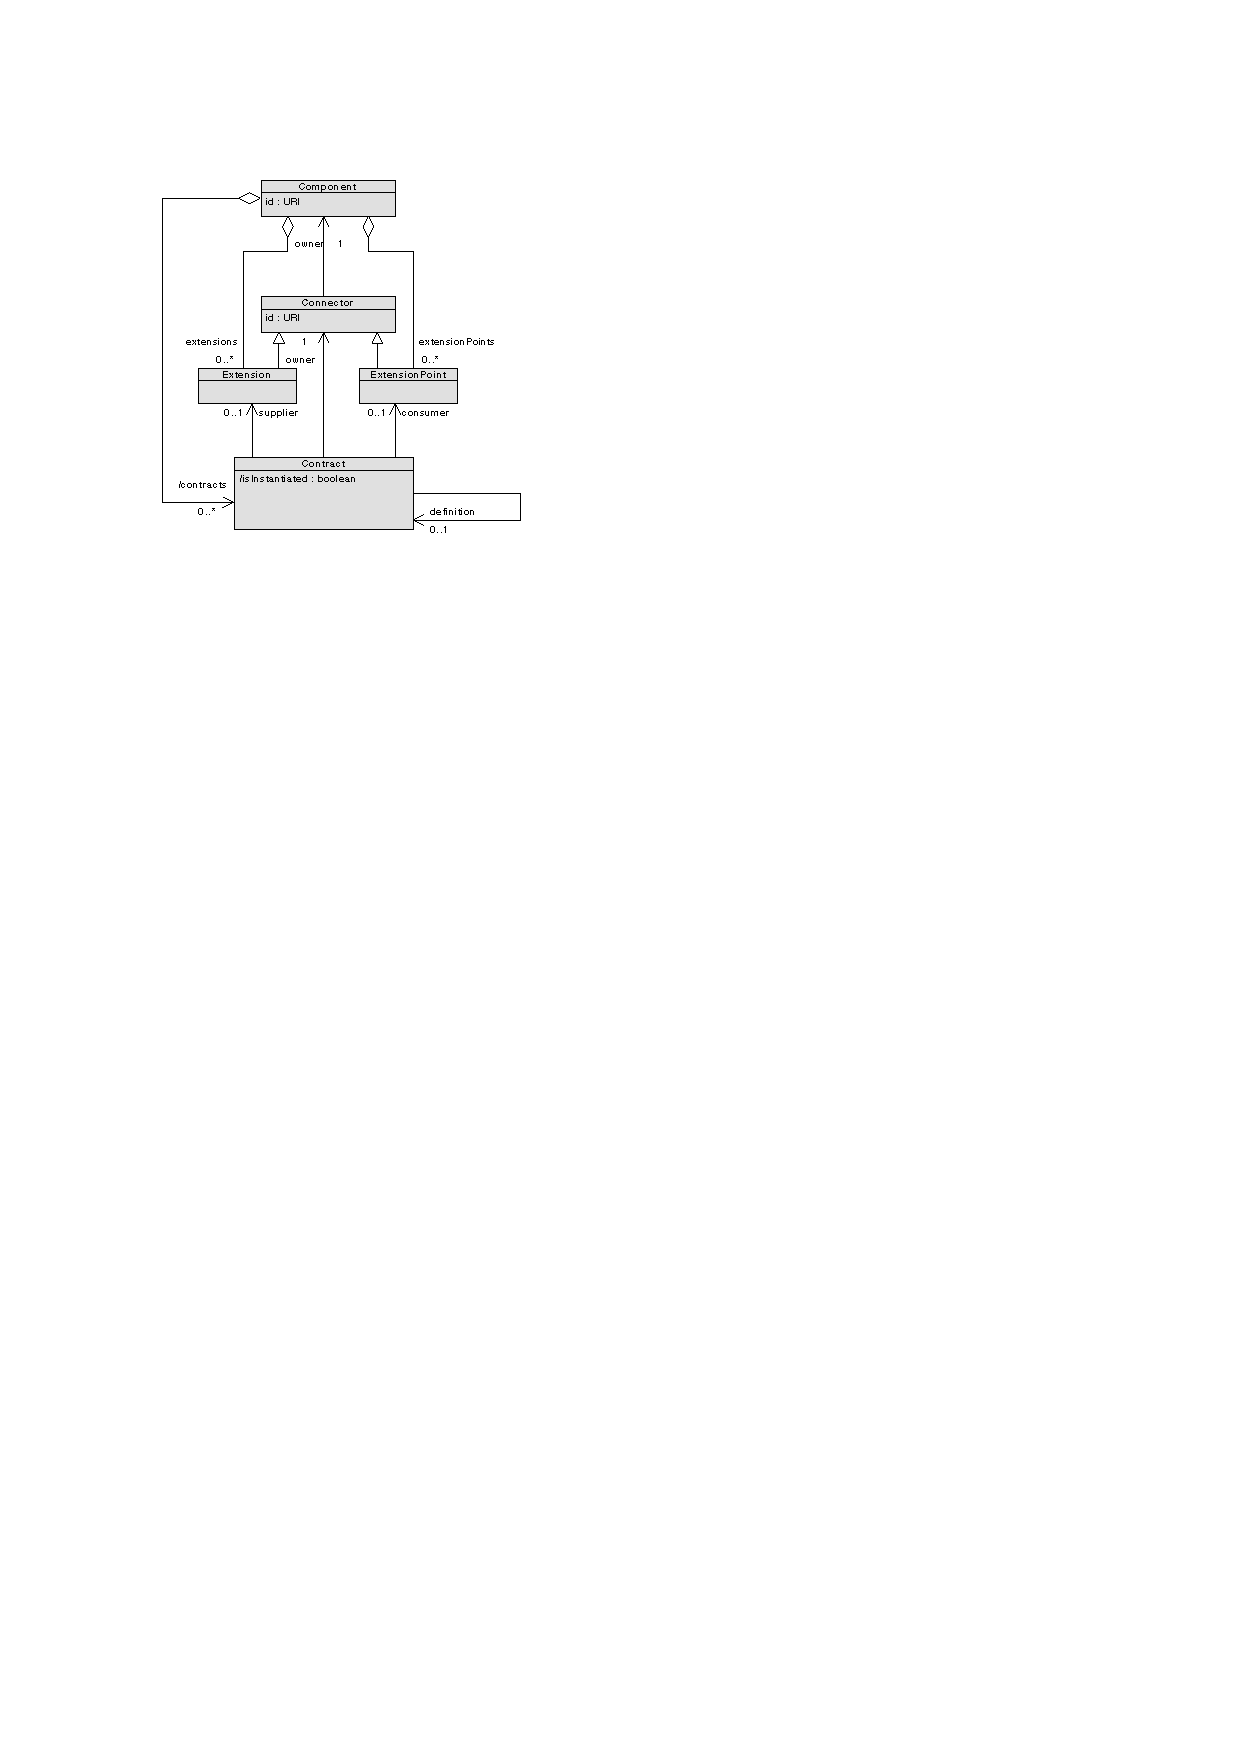
\includegraphics[width=0.5\textwidth]{RoleModel1.pdf}
  \caption{Treaty Structure}
  \label{fig:treatyStructure}
\end{figure}

Figure \ref{fig:treatyStructure} depicts the Treaty model. This model is simplified, in particular, the type hierarchy for \texttt{Condition} representing complex conditions is missing. Treaty supports the a posteriori association of contracts with components. 
This is achieved by using special legislator (contract owner) components that provides contracts for other components.  There are numerous use cases for this, including context-depended contracts and retrofitting existing component-based systems for verification\footnote{See \url{http://www-ist.massey.ac.nz/jbdietrich/treaty/treatyout/index.html} for an experiment where Eclipse has been retrofitted with contracts and verified against these contracts.}.   
 
The Treaty implementation for Eclipse also supports the dynamic composition of contract vocabularies \cite{Treaty.JOT2009}. The use case used to motivate this feature is the following. Assume a company provides a business reporting tool based on the Velocity template engine. They want to allow customers to plug-in in their own reporting templates by providing components supplying resources of the respective type. The type is \texttt{MyReportingTemplate}, a subtype of Velocity Template with restrictions on the variables that can be used in the template - these are exactly the variables the application can bind when the report is generated. To capture this  in a contract, a new resource types \texttt{MyReportingTemplate} must be introduced. This would be part of the reporting tool, and used to safeguard the tool against faulty extensions.  In Treaty, this is called a \textit{vocabulary contribution}. A vocabulary contribution defines new types, properties and relationships, their relationships to other types, properties and relationships, and their semantics. For instance, the vocabulary contribution would provide the semantics represented as a script that loads a resource and checks it by parsing it with a Velocity parser and checking the variables found in the template against a predefined static list of symbols. If the \texttt{MyReportingTemplate} was declared as sub type of \texttt{VelocityTemplate} provided by another contribution, the type reasoner could be used to delegate part of the check to the contribution defining \texttt{VelocityTemplate}. 

The fact that different components can play different roles with respect to a given contract creates dependencies that need to be carefully taken into account when verification in dynamic component models is considered. For instance, if a component $C_1$ provides a contract for (an extension point of) another component $C_2$, the the contract  can only be checked if $C_2$ is present. I.e., there is a runtime dependency between $C_1$ and $C_2$. This dependency is implicit,
but can be made explicit when the components are designed. E.g., OSGi support direct dependencies between bundles\footnote{Declared using the \texttt{Require-Bundle} header.} as well as (less explicit) dependencies through versioned packages\footnote{Declared using the \texttt{Import-Package} and \texttt{Export-Package} headers, respectively.}. A similar dependency exists between components providing contracts and components providing vocabularies for these contracts. 
 


\section{Active Treaty}
\label{section:activeTreaty}

One of the main challenges of verifying dynamic component models is that their configuration is changing at runtime. It is therefore difficult to predict the behaviour of these systems by using static verification (such as unit testing) on pre-deployment snapshots. These snapshots can only cover a small subset of possible runtime configurations, and will therefore not be able to detect many faults resulting from component configuration problems. However, the situation can 
be improved by repeating verification on snapshots taken whenever the configuration changes. This is facilitated by the fact that many dynamic component models support component lifecycle  events indicating lifecycle changes. 
An example lifecycle model for OSGi components is shown in Figure \ref{fig:osgiStates} \cite{OSGI42Core}. OSGi containers fire \texttt{BundleEvent} events to notify observers about bundle lifecycle changes. Eclipse has an additional event mechanism for plug-ins on top of the OSGi mechanism. The \texttt{IExtensionRegistry} fires events when extensions and extension points of Eclipse plug-ins have been added or have been removed. These events can be captured by \texttt{IRegistryEventListener} implementations. Furthermore, the \textit{Eclipse Equinox} \cite{EclipseEquinox} OSGi implementation provides the \texttt{BundleWatcher} interface to capture similar events than \texttt{BundleEvent} events.

\begin{figure}[b]
  \centering
  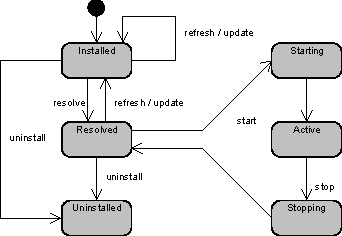
\includegraphics[width=0.5\textwidth]{OSGiStates.pdf}
  \caption{The Lifecycle of an OSGi Component \cite{OSGI42Core}.}
  \label{fig:osgiStates}
\end{figure}

We propose to use these listeners and events to trigger contract verification. In particular, we propose to add the verification triggers to contracts themselves to make the verification policy configirable. We also propose to add the actions to be executed 
upon verification results to the contracts. I.e., we propose to use Event-Condition-Action (ECA) rules to represent contracts. To do this, the following issues need to be addressed:

\begin{enumerate}
  \item An extended syntax for contracts
  \item Semantics of events and actions
  \item Dependency Management
\end{enumerate}


\subsection{Contract Syntax}

In \cite{Treaty.JOT2009} we presented a simple example for a Treaty contract to precise the relationship between a component that prints
dates (clock view) and a component that provides a date formatting service (date to string). This contract is shown in Listing \ref{lst:clock01} (class names are shortened). The contract can be separated into three sections: a \textit{consumer}, a \textit{supplier} and a \textit{constraints section}. The consumer and supplier sections define the resources provided by the components playing the consumer and the supplier role in the contract, respectively. The constraints section defines the constraints that shall be checked during the contract's verification. For further details the reader is referred to \cite{Treaty.JOT2009}.

\begin{figure}[htbp]
\lstset{ 
  language=XML,
  caption=A contract for the clock example.,
  label=lst:clock01
}
\lstinputlisting{clock01.contract}
\end{figure}

To extend Treaty contracts to ActiveTreaty contracts, we had to support a possibility to define events or actions in respect to support the expression of ECA rules in Treaty. Thus, we introduced two new sections, a \textit{trigger} and an \textit{action section}. Listing \ref{lst:clock02} shows an extended contract for the clock example (the already presented sections are not shown completely).

\begin{figure}[htbp]
\lstset{ 
  language=XML,
  caption=A contract for the clock example including triggers and actions.,
  label=lst:clock02
}
\lstinputlisting{clock02.contract}
\end{figure}

In the trigger section, various different triggers for events can be defined that shall cause the verification of the contract. E.g., a trigger can represent the change of the consumer or supplier component's state such as the component's activation (lines 3-4) or installation. ActiveTreaty allows to define multiple triggers for the same contract. They are implicitly connected via \texttt{OR} connectives. Thus, the contract will be verified if any of the described events is triggered. Currently, ActiveTreaty does not allow the composition of events and the use of event calculus to keep the contract language and its verification as simple as possible.

The action section allows the definition of multiple actions that shall be performed either if the contract is violated or verified successfully. ActiveTreaty separates between \textit{on success} and \textit{on failure} actions. E.g., an action can be the logging of a message, warning or exception (lines 5-8) or the deactivation (lines 9-10) or uninstallation of a component. In ActiveTreaty actions are implicitely connected via \texttt{AND} connectives. Thus, if the contract is verified successfully, all on success actions are performed, if the contract's verification fails all on failure actions are performed.
	


\subsection{Event and Action Syntax} 

Similar to the implementation of contract vocabularies which allows to extend the syntax of Treaty contracts with new resource and condition types \cite{Treaty.JOT2009}, the trigger and action types are implemented in an open way and can be extended by context-specific implementations or extensions of ActiveTreaty.

\begin{figure}[htbp]
  \centering
  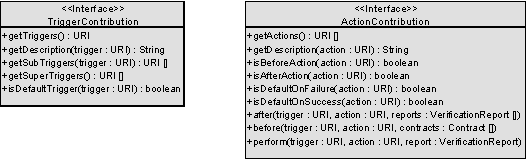
\includegraphics[width=0.8\textwidth]{ContributorModel1.pdf}
  \caption{Trigger and Action Contribution in ActiveTreaty.}
  \label{fig:contribution}
\end{figure}

Figure \ref{fig:contribution} shows the interfaces \texttt{TriggerContribution} and \texttt{Action\-Con\-tri\-bu\-tion} that are used by ActiveTreaty to describe sets of existing triggers and actions, respectively. Triggers and actions are both defined as URIs and do not contain further information about themselves. Nevertheless, the trigger and action contributions provide a method to return a description that contains more information about a trigger or action. Furthermore, triggers can be defined hierarchically. E.g., a trigger \texttt{BundleStarted} could have the sub triggers \texttt{ConsumerBundleStarted} and \texttt{SupplierBundleStarted}. Action types cannot be defined hierarchically because actions must always be declared specifically. On the one hand a contract's trigger can be described abstractly, meaning the contract should be verified if any of the sub trigger events is caused. On the other hand a contract's action cannot be declared abstractly. We have to specify which specific actions we want to execute after the contract's verification and cannot execute abstract actions.

\subsubsection{Default Triggers and Actions}

ActiveTreaty supports triggers to be defined as \textit{default triggers}. Default triggers are used to specify triggers that can cause a contract's verification although the trigger is not declared in the contract. This is useful to define triggers that can be used to verify all selected contracts--e.g., caused by a GUI component that displays a set of contracts and provides such an operation. In ActiveTreaty, \textit{default actions} can be defined as well, although actions can have up to four different kinds of default states:

\begin{enumerate}
	\item Actions can be declared as default before the verification of a set of contracts (\textit{before action}). E.g., an action to log a message how many contracts will be verified caused by a specific trigger.
	\item Actions can be declared as default after the verification of a set of contracts (\textit{after action}). E.g., to log a message how many contracts have been violated during a triggered verification or to show a similar message in a GUI dialog.
	\item Actions can be declared as default after a contract's successful verification (\textit{default on success}). E.g., to log a message that the contract has been verified successfully.
	\item Actions can be declared as default after a contract's failed verification (\textit{default on failure}). E.g., to log a warning including the verification's stack trace.
\end{enumerate}

Please note, that before and after actions cannot be defined in a contract itself but only in an action contribution. A contract can only declare its on success and on failure actions.

\subsubsection{Contribution Composition}

Both trigger and action contributions come with a default implementation that implements the \textit{Composite Pattern} \cite{GangOf4} allowing to implement the contributions hierarchically and to extend and vary them dynamically during runtime.

\subsubsection{How to trigger Events}

If a trigger contribution provides event types, the trigger contribution is also responsible to delegate these events to the \textit{treaty contract verifier} if they occur. Thus, a trigger contribution knows a list of event listeners that must be informed if any of its provided events occur. 

The prototypical ActiveTreaty implementation for Eclipse provides trigger types such as \texttt{BundleStarted} and \texttt{BundleStopped}. To delegate these events, the bundle trigger contribution implements the interface \texttt{org.osgi.framework.Bun\-dle\-Lis\-te\-ner}. Each time, the state of a bundle changed, the trigger contribution informs its event listeners about the occurred event by sending the URI of the specific trigger type and a set of all contracts that must be verified caused by this trigger\footnote{E.g., for a \texttt{ConsumerBundleStarted} event the trigger contribution requests the contract registry of ActiveTreaty for Eclipse to collect all contracts whose consumer component equals to the bundle that has been started. If at least one contract fulfilling this condition is found, the verification is triggered by notifying the trigger contribution's event listeners.}. During startup, the triggered verifier of ActiveTreaty for Eclipse registers itself as a listener of the trigger contributions to be aware of all triggered events.

\subsubsection{How to perform Actions}

To perform the different action types of an action contribution, the action contribution has to implement three methods that are called by the triggered verifier of ActiveTreaty. One method is used to perform actions before a set of contracts is verified (\texttt{before(..)}), another method is used to perform actions after a set of actions is verified (\texttt{after(..)}). The third method exists to perform the on success and on failure actions of a contract's verification result (\texttt{perform(..)}).

\subsubsection{Ontology-based Implementation}

Both action and trigger contributions can be implemented by extending an ontology-based abstract implementation that uses an OWL ontology to reason on the provided types, their descriptions, inheritance relationships and the possible different default settings. These ontology-based implementations are similar to the implementation used for ontology-based contract vocabularies \cite{Treaty.JOT2009}.

\subsubsection{Dynamic Contributions}

The new prototypical implementation of ActiveTreaty for Eclipse is able to update its contributions dynamically. All different contributions (vocabulary, trigger and action contributions) can be composed of multiple contributions that are registered at ActiveTreaty for Eclipse via extension points. ActiveTreaty for Eclipse manages the contributions dynamically and adds and removes them if their providing extensions are added to or removed from the \texttt{IExtensionRegistry}.


\subsection{Dependency Management}

As briefly discussed earlier in this section, the management of dependencies between components having different roles with respect to a contract is a problem that must be addressed when managing contracts in dynamic component systems. We attempt to solve the problem by formally defining the roles, and then defining dependency constraints between these roles. 

\begin{figure}[t]
  \centering
  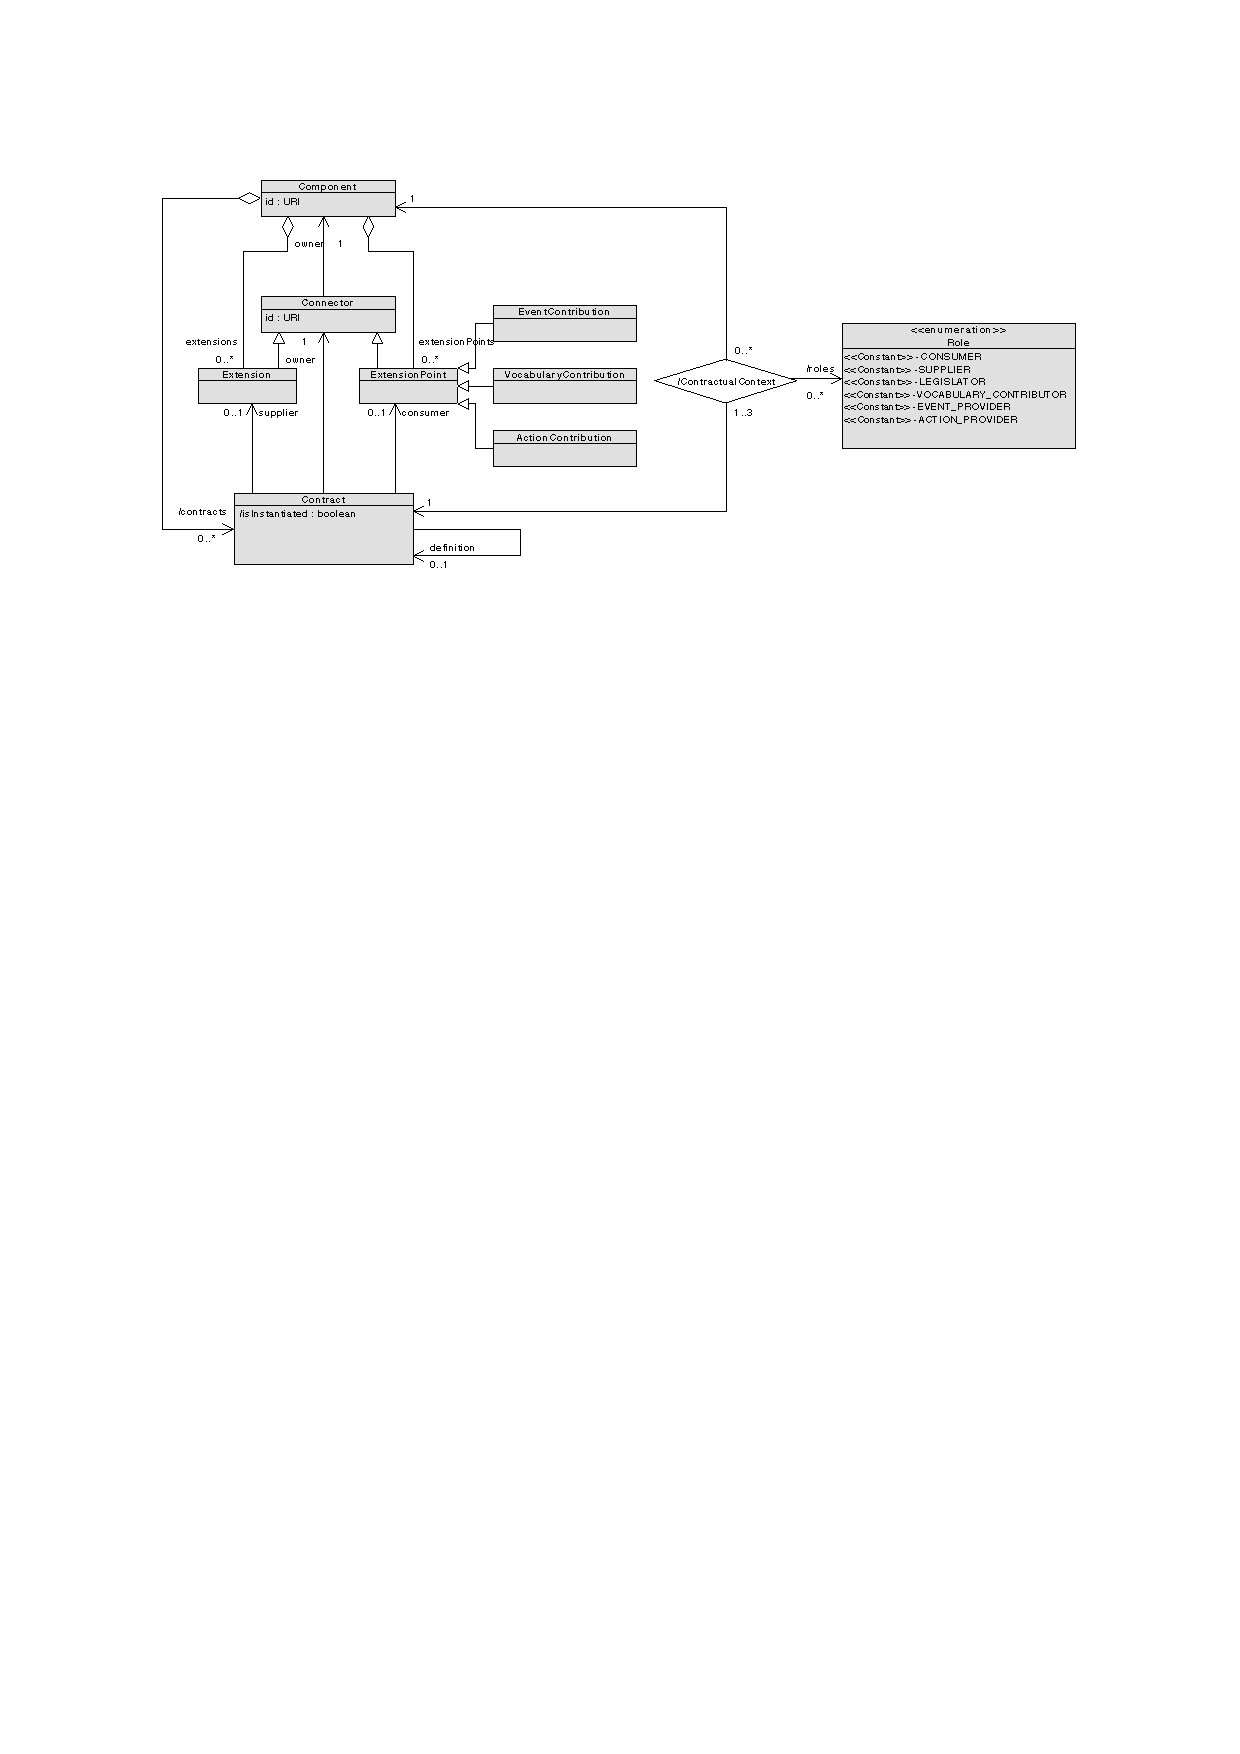
\includegraphics[width=1.0\textwidth]{RoleModel2.pdf}
  \caption{Active Treaty and Contract Roles}
  \label{fig:roles}
\end{figure}

The roles classify relationships between contracts and components. In the model (Figure \ref{fig:roles}), these roles can be introduced as attributes on a derived relationship \texttt{ContractualContext} between contracts and components. The use of roles is similar to how roles are used in \textit{design patterns} \cite{GangOf4} \cite{riehle:roleModels}. Here, a class can play a role like factory or product in the context of a certain (factory) pattern instance. However, a class can be a factory in the context of factory instance 1, and a product in the context of factory instance 2. The precise definition of the associations can be defined using the Object Constraint Language (OCL) \cite{OCL20} as follows. 

\lstset{ language=OCL }
\lstinputlisting{constraints.ocl}
% TODO rules to define event and action contributors are still missing.
% perhaps take out EXTERNAL_CONTRIBUTOR to save some space.
% TODO perhaps use logic instead of OCL to sace some space.

Using these definitions, each contract gives rise to a legislator component and sets of consumers, suppliers, legislators, and vocabulary, event and action contributors. To execute a contract, the following dependencies must be satisfied for each component in the respective role: 

\begin{itemize}
  \item Legislator dependsOn VocabularyContributor
  \item Legislator dependsOn EventContributor
  \item Legislator dependsOn ActionContributor
  \item Legislator dependsOn Consumer
\end{itemize}

% TODO Claas: I'm not sure but I think that in Eclipse every supplier depends on its consumer to know the extension points. %
In many cases, the supplier also depends on the Consumer. An example where this is the case is if the consumer describes a service to be provided by a supplier using a (Java) interface. The supplier needs to provide a class implementing these interface, and needs access to the interface to do this. E.g., in OSGi, the supplier bundle would need access to the class path of the consumer. 

Dependency means that the respective component is available. Availability means that the resources of the component are available. In case of OSGi, this means that a bundle has been installed, resolved and either has been or can be activated. 



\section{A Case Study: Adding Active Contracts to Eclipse}
\label{section:caseStudy}

Points of interest:

\begin{itemize}
	\item which events do we actually implement
  \item discuss OSGi vs Eclipse events
  \item describe global (system) events -> VerifyAll
  \item describe effects of lazy loading in Eclipse
\end{itemize}


\section{Conclusion}
\label{section:conclusion}

We have presented ActiveTreaty, a contract framework for software components based on ECA rules. The proof-of-concept implementation based on Eclipse shows such that this framework can be easily added to an existing component model and can be used to safeguard evolving component assemblies by triggering verification whenever assemblies change. 

There are some open questions though. The actions used in our implementation so far are fairly simple - user notification and logging. While this is useful, it would be desirable to go one step further and to use corrective actions.  In particular actions such as uninstalling faulty components and roll-back component upgrades. However, this causes another problem. Actions interferring with the lifecycle of components will indirectly trigger lifecycle events. These events can trigger new contracts and the system could go into infinite loops. Therefore, verification of contracts is needed. One way of doing this is to build a dependency graph between actions and events and check this graph for circular dependencies. 

The events used so far in ActiveTreaty are flat. The expressive of the contract language could be increased by allowing complex events such as events composed using event algebras. 

TODO more


\subsection{Future Works}

\subsubsection{OCL vocabulary contribution}

Although ActiveTreaty now provides ECA rules powerful enough to describe different events such as component life-cycle changes, the implementation still misses some features for more complex trigger types. In a case study \cite{DAWilke} we investigated if and how it is possible to extend ActiveTreaty for Eclipse by providing a new vocabulary contribution that introduces conditions to define OCL constraints \cite{OCL20} on interfaces defined as resources in contracts. To verify such \textit{design by contract} \cite{DesignByContract,meyerOOSC} contracts, further information is required for the contracts' verification.

E.g., if we want to verify a postcondition on the operation \texttt{Date\-for\-mat\-ter\linebreak[0].for\-mat(Date)}, we have to know which argument (date object) was given as parameter of the operation's invocation and also the value in that the invocation resulted. Thus, triggers need to provide a context information for their listeners that can be used to describe such information. Future work will investigate how this context information can be shipped to the verifier and the vocabularies in an easy and generic way.

TODO Probably more

\begin{itemize}
	\item implement (Active)Treaty for other component models
\end{itemize}



%TODO change to LNCS style
\bibliography{bibliography}  
    
\end{document}
